\section{Null pointers}

\subsection{``Null pointer assignment'' error of MS-DOS era}

Some oldschoolers may remember a weird error message of MS-DOS era: ``Null pointer assignment''.
What does it mean?

It's not possible to write a memory at zero address in *NIX and Windows OSes, but it was possible to do so in MS-DOS due to absence of memory protection whatsoever.

So I've pulled my ancient Turbo C++ 3.0 (later it was renamed to Borland C++) from early 1990s and tried to compile this:

\begin{lstlisting}
#include <stdio.h>

int main()
{
	int *ptr=NULL;
	*ptr=1234;
	printf ("Now let's read at NULL\n");
	printf ("%d\n", *ptr);
};
\end{lstlisting}

Hard to believe, but it works, with error upon exit, though:

\begin{figure}[H]
	\centering
	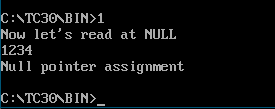
\includegraphics[scale=\NormalScale]{advanced/450_more_ptrs/tc30.png}
	\caption{Ancient Turbo C 3.0}
\end{figure}

Let's dig deeper into the source code of CRT (C runtime) of Borland C++ 3.1, file \IT{c0.asm}:

\begin{lstlisting}
;       _checknull()    check for null pointer zapping copyright message

...

;       Check for null pointers before exit

__checknull     PROC    DIST
                PUBLIC  __checknull

IF      LDATA  EQ  false
  IFNDEF  __TINY__
                push    si
                push    di
                mov     es, cs:DGROUP@@
                xor     ax, ax
                mov     si, ax
                mov     cx, lgth_CopyRight
ComputeChecksum label   near
                add     al, es:[si]
                adc     ah, 0
                inc     si
                loop    ComputeChecksum
                sub     ax, CheckSum
                jz      @@SumOK
                mov     cx, lgth_NullCheck
                mov     dx, offset DGROUP: NullCheck
                call    ErrorDisplay
@@SumOK:        pop     di
                pop     si
  ENDIF
ENDIF

_DATA           SEGMENT

;       Magic symbol used by the debug info to locate the data segment
                public DATASEG@
DATASEG@        label   byte

;       The CopyRight string must NOT be moved or changed without
;       changing the null pointer check logic

CopyRight       db      4 dup(0)
                db      'Borland C++ - Copyright 1991 Borland Intl.',0
lgth_CopyRight  equ     $ - CopyRight

IF      LDATA  EQ  false
IFNDEF  __TINY__
CheckSum        equ     00D5Ch
NullCheck       db      'Null pointer assignment', 13, 10
lgth_NullCheck  equ     $ - NullCheck
ENDIF
ENDIF

...

\end{lstlisting}

The MS-DOS memory model was really weird and probably not worth looking into it unless you're fan of retrocomputing or retrogaming.
One thing we should know that memory segment (included data segment) in MS-DOS is a memory segment in which code or data is stored,
but unlike "serious" OSes, it's started at address 0.

And in Borland C++ CRT, the data segment is started with 4 zero bytes and the copyright string ``Borland C++ - Copyright 1991 Borland Intl.''.
The integrity of the 4 zero bytes and text string is checked upon exit, and if it's corrupted, the error message is displayed.

But why? Writing at null pointer is common mistake in \CCpp, and if you do so in *NIX or Windows, your application will crash.
MS-DOS has no memory protection, so CRT has to check this post-factum and warn about it upon exit.
If you see this message, this mean, your program at some point has written at address 0.

Our program did so. And this is why 1234 number was correctly read: because it was written at the place of the first 4 zero bytes.
Checksum was incorrect upon exit (because the number has left there), so error message has been displayed.

Am I right?
I've rewritten the program to check my assumptions:

\begin{lstlisting}
#include <stdio.h>

int main()
{
	int *ptr=NULL;
	*ptr=1234;
	printf ("Now let's read at NULL\n");
	printf ("%d\n", *ptr);
	*ptr=0; // oops, cover our tracks!
};
\end{lstlisting}

This program works without error message upon exit.

Though method to warn about null pointer assignment is relevant for MS-DOS,
it's probably can be still used in low-cost microcontrollers without memory protection and/or \ac{MMU}.

\subsection{Why would anyone write at address 0?}

But why would sane programmer write a code which writes something at address 0?
It can be done accidentally: for example, a pointer must be initialized to newly allocated memory block and then passed to some function which returns data through pointer.

\begin{lstlisting}
int *ptr=NULL;

... we forgot to allocate memory and initialize ptr

strcpy (ptr, buf); // strcpy() terminates silently because MS-DOS has no memory protection
\end{lstlisting}

Even worse:

\begin{lstlisting}
int *ptr=malloc(1000);

... we forgot to check if memory was really allocated: this is MS-DOS after all and computers had small amount of RAM,
... and RAM shortage was very common.
... malloc() may return NULL, so ptr now is also NULL.

strcpy (ptr, buf); // strcpy() terminates silently because MS-DOS has no memory protection
\end{lstlisting}

\subsection{NULL in \CCpp}

NULL in C/C++ is just a macro which is often defined like this:

\begin{lstlisting}
#define NULL  ((void*)0)
\end{lstlisting}
( \href{https://github.com/wzhy90/linaro_toolchains/blob/8ff8ae680bac04558d10cc9626e12c4c2f6c1348/arm-cortex_a15-linux-gnueabihf/libc/usr/include/libio.h#L70}{libio.h file} )

\IT{void*} is a data type reflecting the fact it's the pointer, but to a value of unknown data type (\IT{void}).

NULL is usually used to show absence of an object.
For example, you have a single-linked list, and each node has a value (or pointer to a value) and \IT{next} pointer.
To show that there are no next node, 0 is stored to \IT{next} field.
Other solutions are just worse.
You may probably have some crazy environment where you need to allocate memory blocks at zero address. How would you indicate absence of the next node?
Some kind of magic number? Maybe -1? Or maybe additional bit?

In Wikipedia we may find this:

\begin{framed}
\begin{quotation}
In fact, quite contrary to the zero page's original preferential use, some modern operating systems such as FreeBSD, Linux and Microsoft Windows[2] actually make the zero page inaccessible to trap uses of NULL pointers. 
\end{quotation}
\end{framed}
( \url{https://en.wikipedia.org/wiki/Zero_page} )

\subsection{Null pointer to function}

It's possible to call function by its address.
For example, I compile this by MSVC 2010 and run it in Windows 7:

\begin{lstlisting}
#include <windows.h>
#include <stdio.h>

int main()
{
	printf ("0x%x\n", &MessageBoxA);
};
\end{lstlisting}

The result is \IT{0x7578feae} and doesn't changing after several times I run it,
because user32.dll (where MessageBoxA function resides) is always loads at the same address.
And also because \ac{ASLR} is not enabled (result would be different each time in that case).

Let's call \IT{MessageBoxA()} by address:

\begin{lstlisting}
#include <windows.h>
#include <stdio.h>

typedef int (*msgboxtype)(HWND hWnd, LPCTSTR lpText, LPCTSTR lpCaption,  UINT uType);

int main()
{
	msgboxtype msgboxaddr=0x7578feae;

	// force to load DLL into process memory, 
	// since our code doesn't use any function from user32.dll, 
	// and it is not imported
	LoadLibrary ("user32.dll");

	msgboxaddr(NULL, "Hello, world!", "hello", MB_OK);
};
\end{lstlisting}

Weird, but works in Windows 7.

This is commonly used in shellcodes, because it's hard to call DLL functions by name from there.
And \ac{ASLR} is a countermeasure.

Now what is really weird, some embedded C programmers may be familiar with a code like that:

\begin{lstlisting}
int reset()
{
	void (*foo)(void) = 0;
	foo();
};
\end{lstlisting}

Who will need to call a function at address 0?
This is portable way to jump at zero address.
Many low-cost cheap microcontrollers also have no memory protection or \ac{MMU} and after reset, they start to execute code at address 0, where some kind of initialization code is stored.
So jumping to address 0 is a way to reset itself.
One could use inline assembly, but if it's not possible, this is portable method.

It even compiles correctly by my GCC 4.8.4 on Linux x64:

\begin{lstlisting}
reset:
        sub     rsp, 8
        xor     eax, eax
        call    rax
        add     rsp, 8
        ret
\end{lstlisting}

The fact that stack pointer is shifted is not a problem: initialization code in microcontrollers usually completely ignores registers and RAM state and boots from scratch.

And of course, this code will crash on *NIX or Windows because of memory protection and even in absence of protection, there are no code at address 0.

GCC even has non-standard extension, allowing to jump to a specific address rather than call a function there: \url{http://gcc.gnu.org/onlinedocs/gcc/Labels-as-Values.html}.

